
\documentclass[12pt, a4paper]{article}
\usepackage[utf8]{inputenc}
\usepackage{graphicx}
\graphicspath{ {./} }

\title{my document}
\author{Hubert Farnsworth}
\date{May 2024}

\begin{document}

\maketitle

We have now added a title, author and date to our first \LaTeX{} document!

% This line here is a comment. It will not be printed in the document.
Some of the \textbf{greatest}
discoveries in \underline{science}
were made by \textbf{\textit{accident}}.

Some of the greatest \emph{discoveries}
in science
were made by accident.

\textit{Some of the greatest \emph{discoveries}
in science
were made by accident.}

\begin{figure}[h]
	\centering
	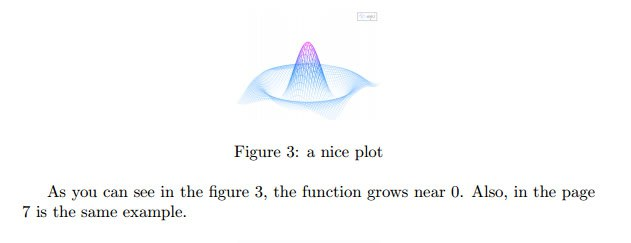
\includegraphics[width=0.25\textwidth]{mesh}
	% Подписывает изображение. При созданиее списка изображений данная подпис.jpg
	\caption{a nice plot}
	% Если необходимо сослаться на изображение внутрии доукумента, необходимо установить метку с помощью данной команды. Метка пронумеруюет изображение и при использовании вместе со сл. командой позволит на него сослаться.
	\label{fig:mesh1}
\end{figure}

As you can see in the figure 
% Этот код будет замещен числом, соответствующим изображению, на которое делается ссылка.
\ref{fig:mesh1}, the function grows near 0. Also, in the page \pageref{fig:mesh1} is the same example.

\textbf{Some of the greatest \emph{discoveries}
in science
were made by accident.}


\includegraphics{photo}
There's a picture from this is pc.

\begin{itemize}
	\item The individual entries are indicated with a black dot, a so-called bullet.
	\item The text in the entries may be of any length.
\end{itemize}

\begin{enumerate}
	\item This is first entry in our list
	\item This list numbers increase with each entry we add
\end{enumerate}

% Для размещения уравнений в режиме встраивание (inline) используют один из следующих разделителей: 
% \( ... \), $ ... $, \begin{matha} ... \end{math}. (Работают они равнозначно)
In physics, the mass-energy equivalence is stated be the equation
$E=mc^2$, discovered in 1905 by Albert Einstein.

% Для отображения есть два варианта:

	%Для вывода уравнений в режиме отображения используйте один из следующих разграничителей: \[ ... \], \begin{displaymath} ... \end{displaymath} или \begin{equation} ... \end{equation}. Применять $$ ... $$ нежелательно, так как он может внести несогласованные интервалы, а также коряво работать с некотороми математическими пакетами.
	%Важно: окружение equation* предоставляется в виде стороннего пакета. Подробнее об этом рекомендую почитать статью по amsmath.

% Без нумерации
The mass-energy equivalence is stated be the equation
\[ E=mc^2 \]
discovered in 1905 by Albert Einstein.

% С нумерацией
In natural units ($c = 1$), the formula expresses the identity
\begin{equation}
E=m
\end{equation}

\end{document}

